\documentclass{bmvc2k}
\usepackage{url}

%% Enter your paper number here for the review copy
% \bmvcreviewcopy{??}

\title{PythonRobotics: a Python code collection of robotics algorithms}

% Enter the paper's authors in order
% \addauthor{Name}{email/homepage}{INSTITUTION_CODE}
\addauthor{Atsushi Sakai}{https://atsushisakai.github.io/}{1}

% Enter the institutions
% \addinstitution{Name\\Address}
\addinstitution{
 University of California, Berkeley\\
 Berkeley, USA
}


\runninghead{arXiv}{Robotics, Artificial Intelligence}

% Any macro definitions you would like to include
% These are not defined in the style file, because they don't begin
% with \bmva, so they might conflict with the user's own macros.
% The \bmvaOneDot macro adds a full stop unless there is one in the
% text already.
\def\eg{\emph{e.g}\bmvaOneDot}
\def\Eg{\emph{E.g}\bmvaOneDot}
\def\etal{\emph{et al}\bmvaOneDot}

%------------------------------------------------------------------------- 
% Document starts here
\begin{document}

\maketitle

\begin{abstract}
This paper describes an Open Source Software(OSS): PythonRobotics\cite{github}.This OSS is a Python code collection of robotics algorithms, especially focusing on autonomous navigation. It aims for beginners of robotics to understand basic ideas of each algorithm. The algorithms which is widely used in academia and industry and practical are selected. Each sample code only depends some standard modules on Python 3.x. In this paper, related works of this project, some key ideas about this OSS project, and brief structure of this repository are introduced. I also discuss future works of this project. 

\end{abstract}

%------------------------------------------------------------------------- 
\section{Introduction}

In recent years, autonomous navigation technologies have received a great deal of attention in many fields. 
For examples, autonomous driving\cite{pathplanning}, drone flight navigation, and other transportation systems.
An autonomous system is a system that can operate for long periods of time without any external control.
To accomplish autonomous navigation, the system needs to know where am I (localization), where is safe (mapping), where to go (path planning), and how to go (control). 
Autonomous navigation needs a wide range of technologies.




However, there are 

In this paper, an Open Source Software(OSS) project: PythonRobotics\cite{github} is described.
It aims for beginners of robotics to understand basic ideas of each algorithm.
It is a code collection of robotics algorithms, especially focusing on autonomous navigation. It is written in Python\cite{python} under MIT license\cite{mit}. 

This paper is organized as follows: Section 2 reviews the related works. The philosophy of this OSS is presented in Section 3. It's repository structure description and some technological backgrounds and simulation results are provided in Section 4. Conclusions and some future works are drawn in Section 5. Section 6 shows acknowledgements for all contributors  in this project. The source code of this paper is provided at \url{https://github.com/AtsushiSakai/PythonRobotics}.


\section{Related works}

There are great references for learning autonomous navigation technologies.

S. Thrun et al, wrote a great text book "Probabilistic robotics" which is a bible of localization, mapping, simultaneous localization and mapping (SLAM) for mobile robotics\cite{PR}.
E. Frazzoli et al. wrote a survey paper about path planning and control for autonomous driving \cite{pathtracking}.
G. Bautista et al. wrote a survey paper focusing on path planning for automated vehicles\cite{pathplanning}.
J. Levinson wrote an overview paper about systems and algorithms towards fully fully autonomous driving\cite{Levinson2011}.

These papers helps readers to learn state of the arts autonomous technologies.
However, it is difficult to understand the basic ideas of the technologies for beginners of robotics, because these papers doesn't include implementation examples such as sample codes.



Udacity Inc, which is a online learning company founded by S. Thrun, et al, is providing great online courses of autonomous navigation and autonomous driving \cite{udacity}.



\section{Philosophy}
In this section, the philosophy of this project is described.
This project based on three philosophies.

The first one is that the codes have to be easy to read for understanding each algorithm's basic idea.
This project aims for beginners of robotics to understand basic ideas of each algorithm. 
Therefore, the code have to be easy to read and understand the algorithm.
Programming language, Python\cite{python} is adopted in this project because it has good code readability and it allows us to focus on algorithm itself.
Python has great libraries for matrix operation, mathematical and scientific operation, and visualization.
These libraries also allows us to focus on algorithm itself.

The second one is the algorithms which is widely used in academia and industry and practical are selected.
For example, Kalman filters and particle filter for localization, grid mapping for mapping, dynamic programming based approaches and sampling based approaches for path planning, and optimal control based approach for path tracking.

The last philosophy is minimum dependency.
It allows us to use the codes easily and to convert the codes to other programming languages such as C++, Java for practical usage.
Each sample code only depends some modules on Python3 as bellows.

\begin{itemize}
 \item numpy\cite{numpy} for matrix operation
 \item scipy\cite{scipy} for mathematics, science, and engineering computing
 \item matplotlib\cite{matplotlib} for visualization
 \item pandas\cite{pandas} for data analysis
 \item cvxpy\cite{cvxpy} for convex optimization
\end{itemize}

These modules are OSS and could be used for free. This repository doesn't include any commercial software.


\section{Repository structure}

In this section, the brief structure of this project is described.

This repository has five directories which means five technical categories in autonomous navigation, Localization, Mapping, SLAM, Path planning, and Path tracking. Each directory includes several directories which has each sample code with different algorithms.

In the following subsections, some algorithms and some simulation examples described.

\subsection{Localization}

Localization is an ability of a robot to know it's position and orientation with sensors such as GNSS and IMU.
In localization, Bayesian Filters such as Kalman filters, histogram filter, and particle filter are widely used\cite{PR}.
This repository includes some sample codes using these algorithms.
Fig.\ref{fig:localization} shows localization simulation results using histogram filter and particle filter.

\begin{figure}
\begin{tabular}{cc}
\bmvaHangBox{\fbox{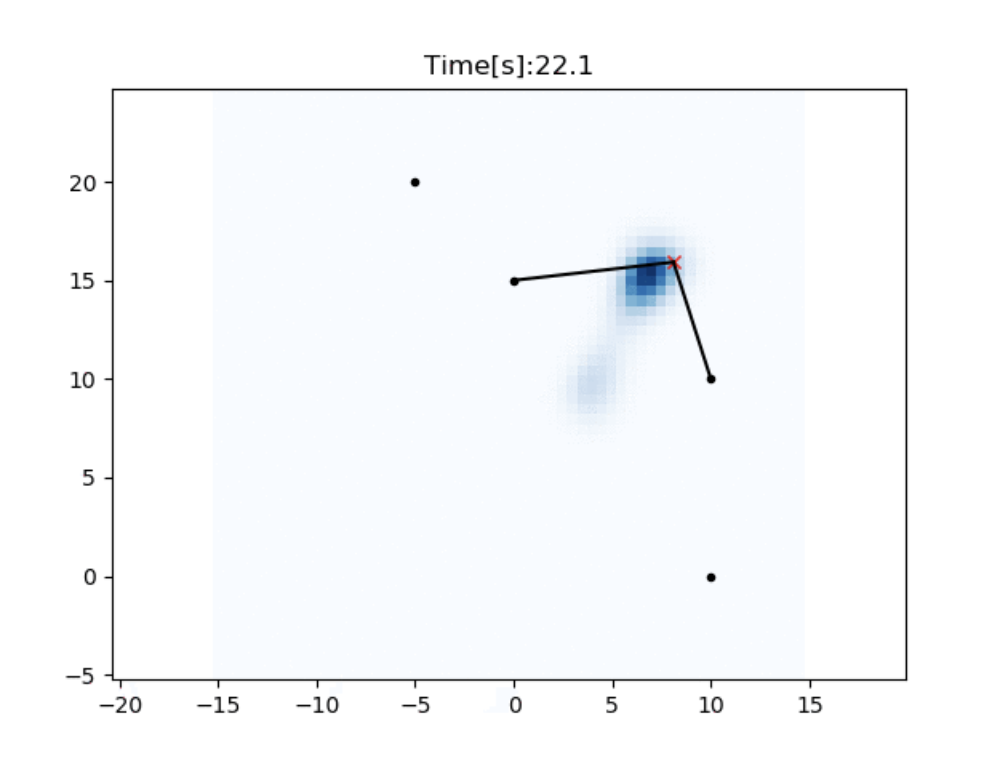
\includegraphics[width=5.9cm]{images/localization1.png}}}&
\bmvaHangBox{\fbox{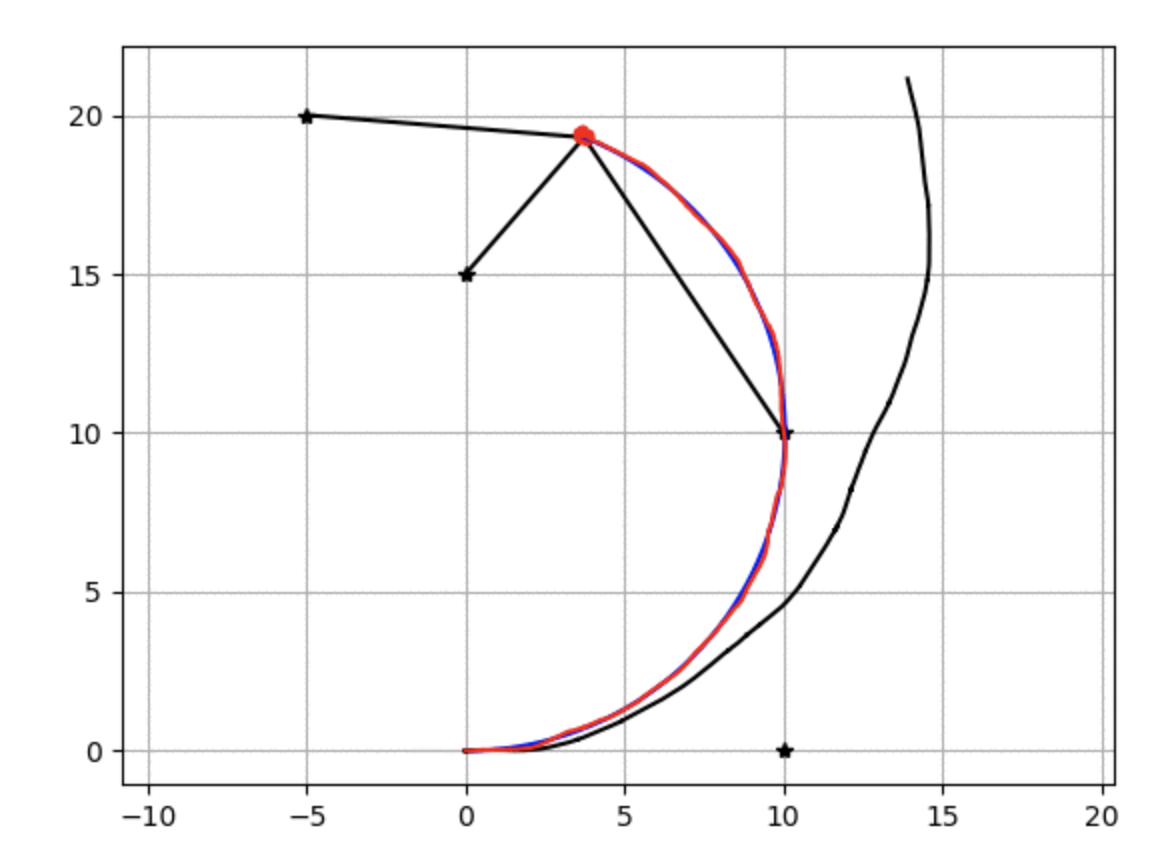
\includegraphics[width=6.2cm]{images/localization2.png}}}\\
Histogram filter&Particle filter
\end{tabular}
\caption{Localization simulation results}
\label{fig:localization}
\end{figure}

\subsection{Mapping}
Mapping is an ability of a robot to understand surroundings with sensors such as LIDAR and imaging sensor.
Robots have to recognize obstacle positions and it' shape for obstacle avoidance.
In mapping, Grid map, machine learning algorithms are widely used\cite{PR}\cite{PRML}.
This repository includes some sample codes using these algorithms.
Fig.\ref{fig:mapping} shows mapping simulation results using Grid mapping with 2D ray casting and 2D object clustering with k-means algorithm.

\begin{figure}
\begin{tabular}{cc}
\bmvaHangBox{\fbox{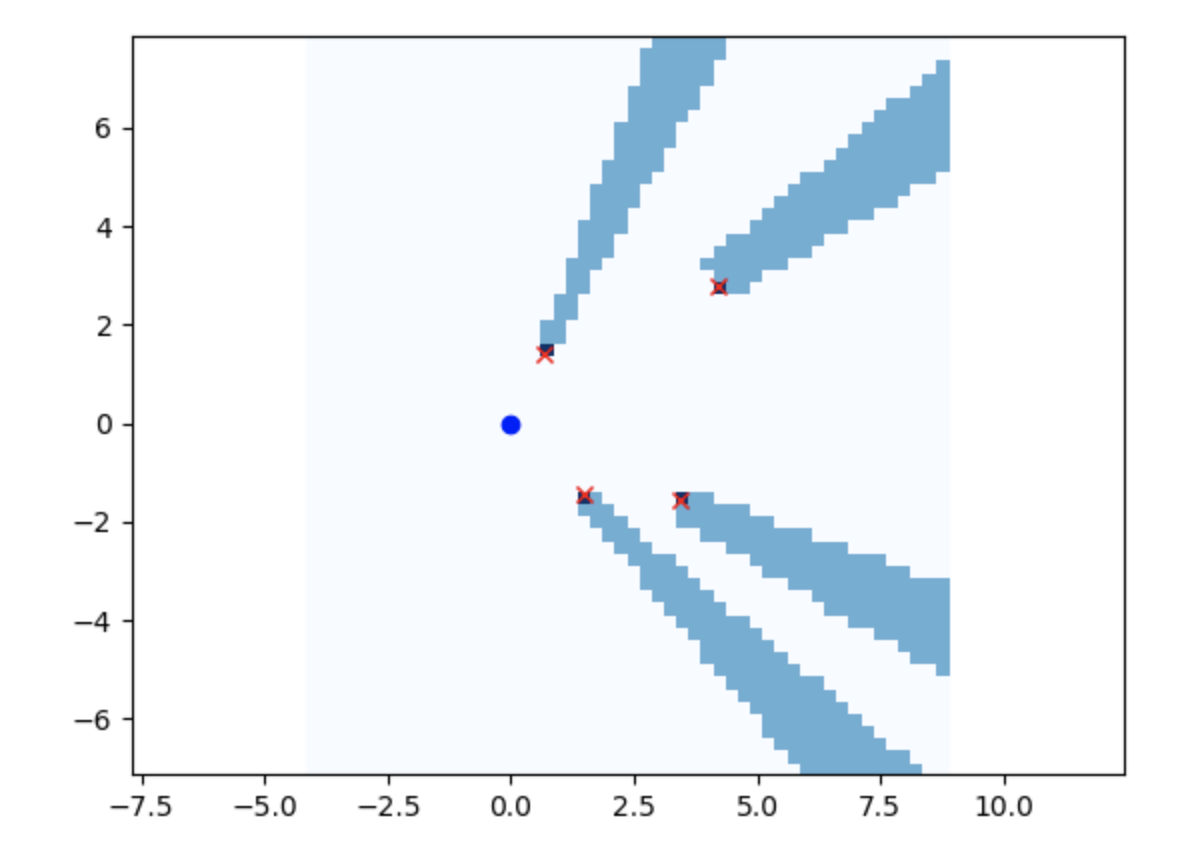
\includegraphics[width=6.0cm]{images/mapping1.png}}}&
\bmvaHangBox{\fbox{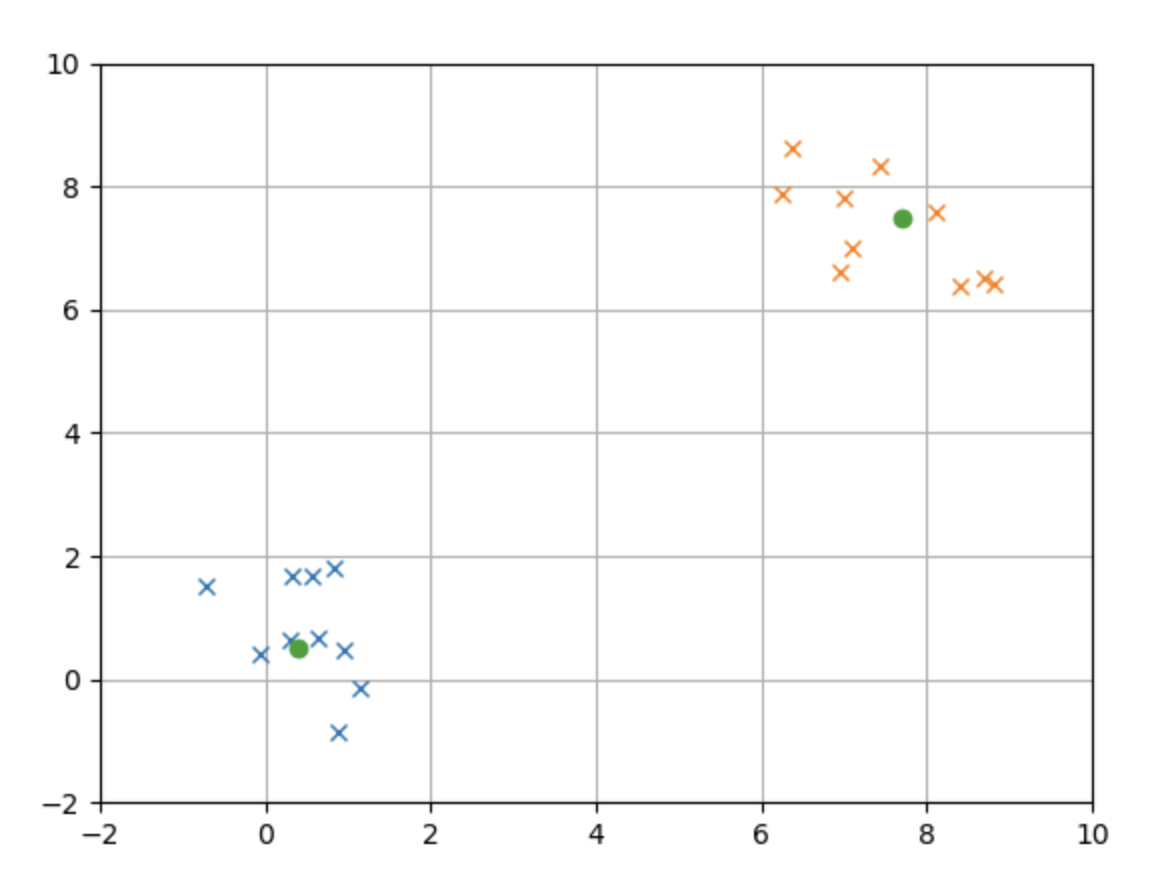
\includegraphics[width=5.7cm]{images/mapping2.png}}}\\
Grid mapping with 2D ray casting&2D object clustering with k-means algorithm
\end{tabular}
\caption{Mapping simulation results}
\label{fig:mapping}
\end{figure}

\subsection{SLAM}
Simultaneous Localization and Mapping: SLAM is an ability of a robot to estimate the pose of a robot and the map of the environment at the same time.
SLAM problem is hard to solve, because a map is needed for localization and a good localization is needed for mapping, which is a kind of chicken and egg problem.
Popular SLAM solution methods include the extended Kalman filter, particle filter, and Fast SLAM algorithm\cite{PR}.
This repository includes some sample codes using these algorithms.
Fig.\ref{fig:slam} shows SLAM simulation results using extended kalman filter and results using FastSLAM2.0\cite{PR}.

\begin{figure}
\begin{tabular}{cc}
\bmvaHangBox{\fbox{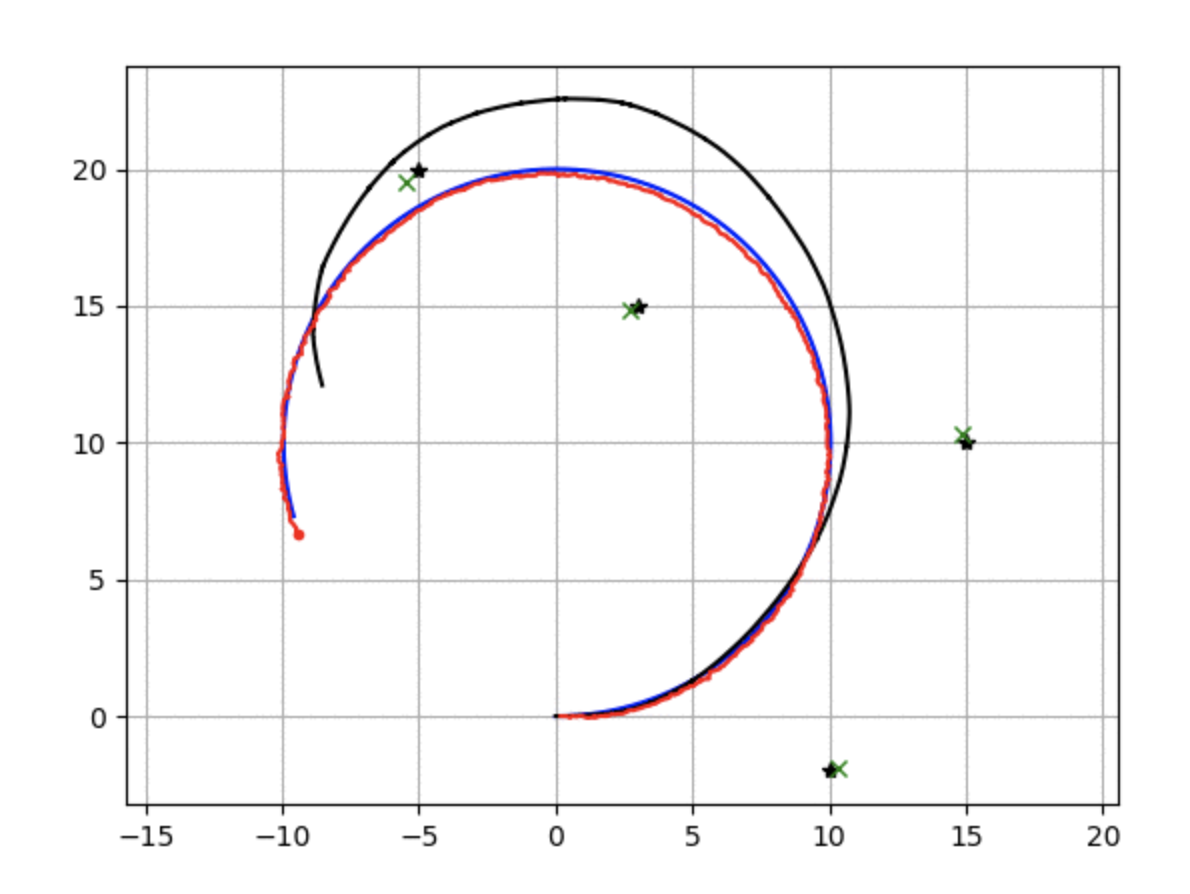
\includegraphics[width=6.0cm]{images/slam1.png}}}&
\bmvaHangBox{\fbox{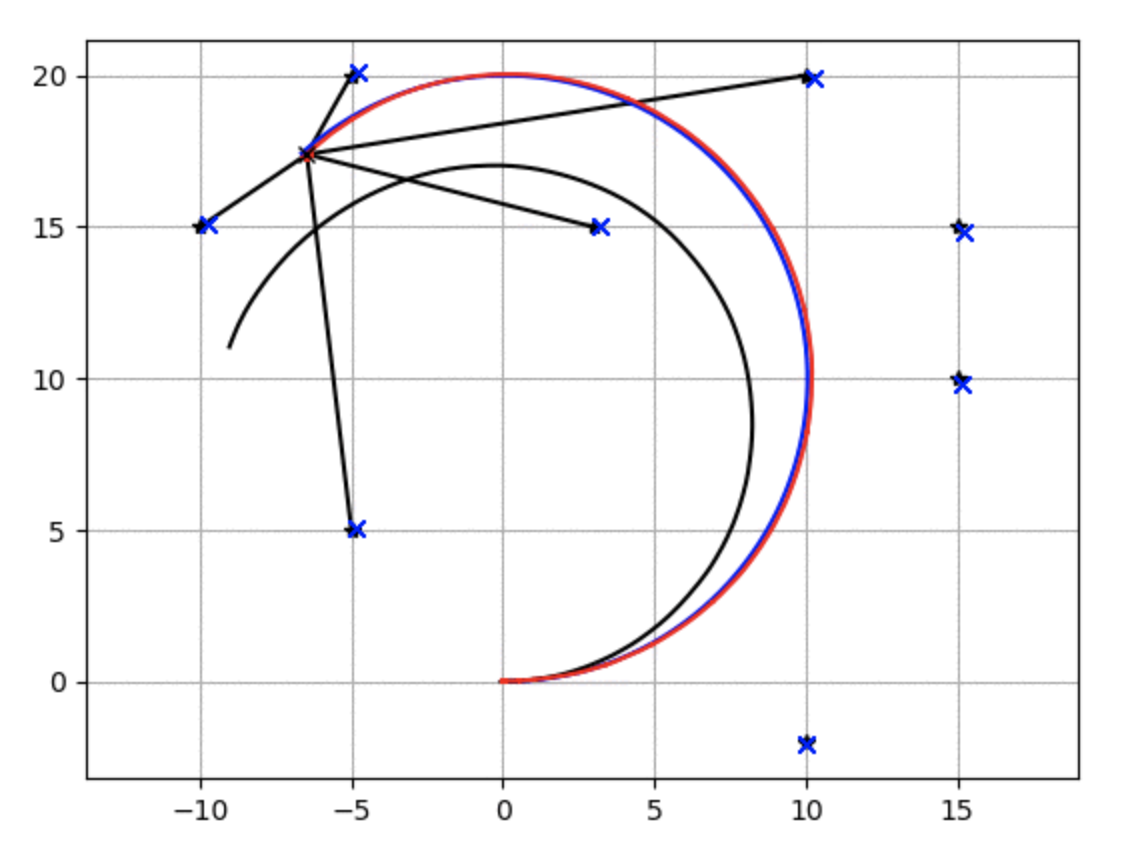
\includegraphics[width=6.0cm]{images/slam2.png}}}\\
Extended Kalman Filter based SLAM & FastSLAM 2.0 based SLAM
\end{tabular}
\caption{SLAM simulation results}
\label{fig:slam}
\end{figure}

\subsection{Path planning}

Path planning is an ability of a robot to search feasible and efficient path to the goal.
The path have to satisfy some constraints based on movement model and obstacle positions and optimize some objective function such as time to goal and distance to obstacle etc.
In path planning, dynamic programming based approaches and sampling based approaches are widely used\cite{pathplanning}.
This project includes some sample codes using these algorithms.
Fig.\ref{fig:pathplan} shows potential field path planning and LQR-RRT* path planning\cite{lqrrrt}.

\begin{figure}
\begin{tabular}{cc}
\bmvaHangBox{\fbox{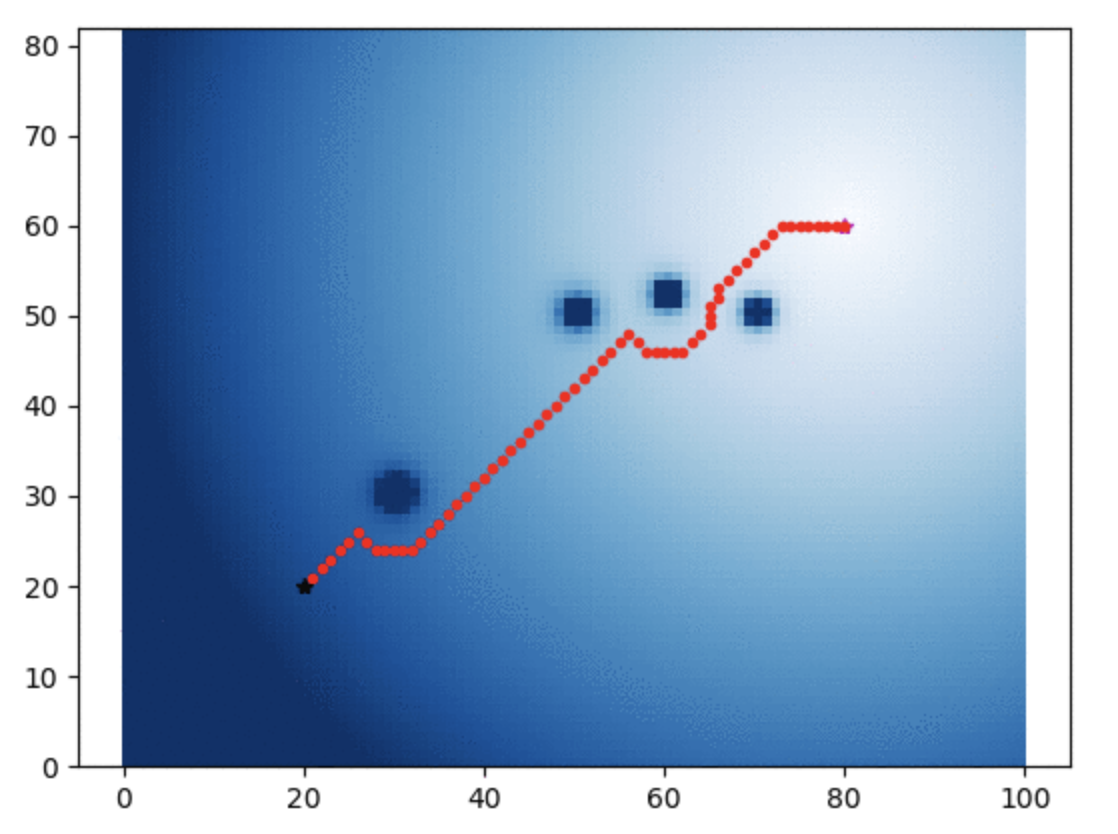
\includegraphics[width=6.0cm]{images/pathplan1.png}}}&
\bmvaHangBox{\fbox{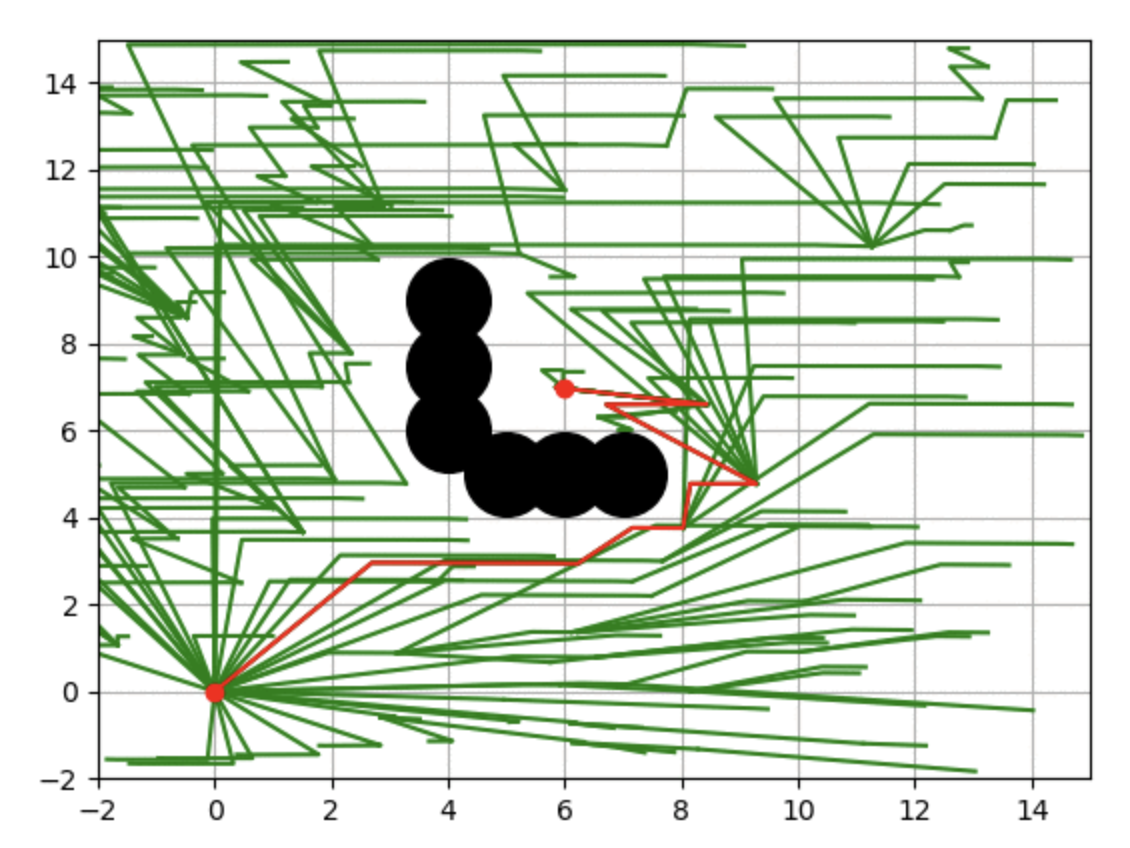
\includegraphics[width=6.0cm]{images/pathplan2.png}}}\\
Potential Field path planning & LQR-RRT* path planning\cite{lqrrrt}
\end{tabular}
\caption{Path planning simulation results}
\label{fig:pathplan}
\end{figure}

\subsection{Path tracking}
Path tracking is an ability of a robot to follow the reference path from path planning algorithms.
The role of the path tracking controller
is to stabilize to the reference path or trajectory which has modeling error and other forms of uncertainty. 
In path tracking, feedback control techniques and optimization based control techniques are widely used\cite{pathplanning}.
This project includes some sample codes using these algorithms.
Fig.\ref{fig:pathplan} shows Rear wheel feedback steering control and PID speed control and iterative linear model predictive path tracking control\cite{lqrrrt}.

\begin{figure}
\begin{tabular}{cc}
\bmvaHangBox{\fbox{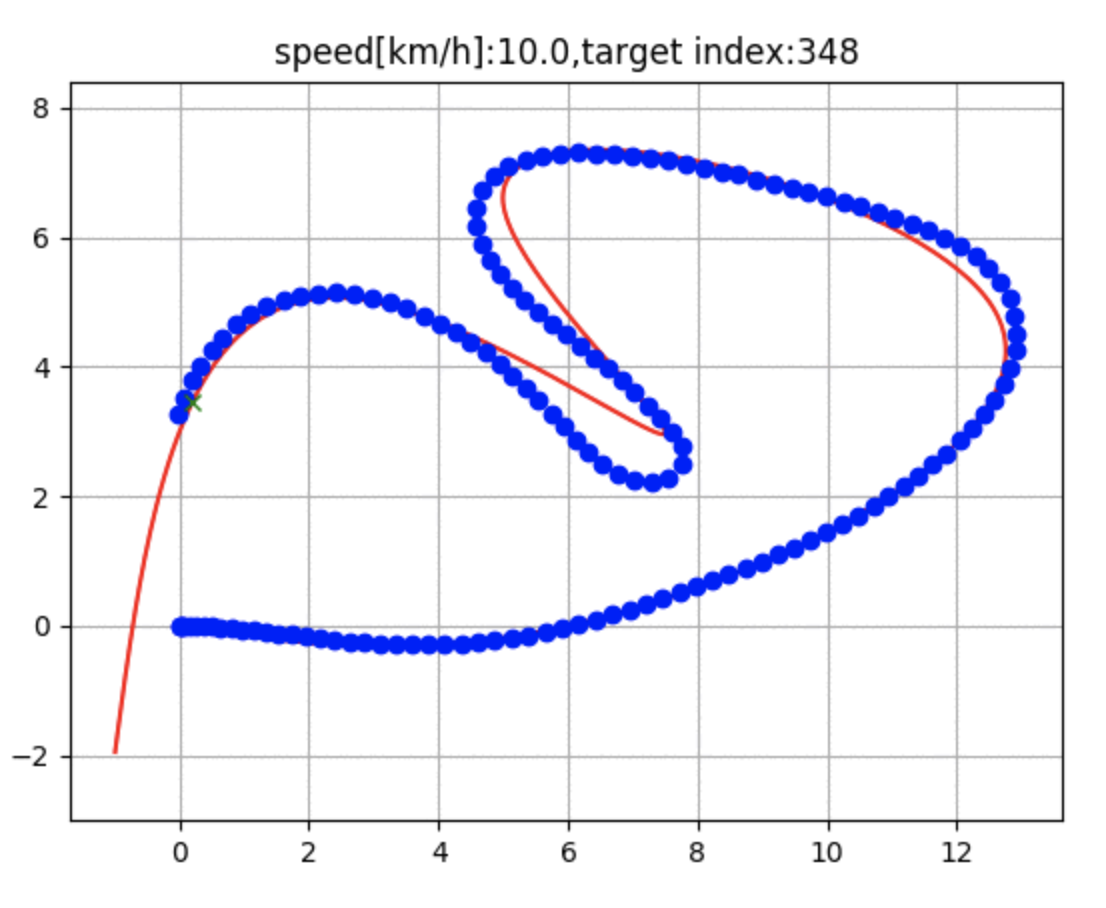
\includegraphics[width=6.0cm]{images/path_tracking1.png}}}&
\bmvaHangBox{\fbox{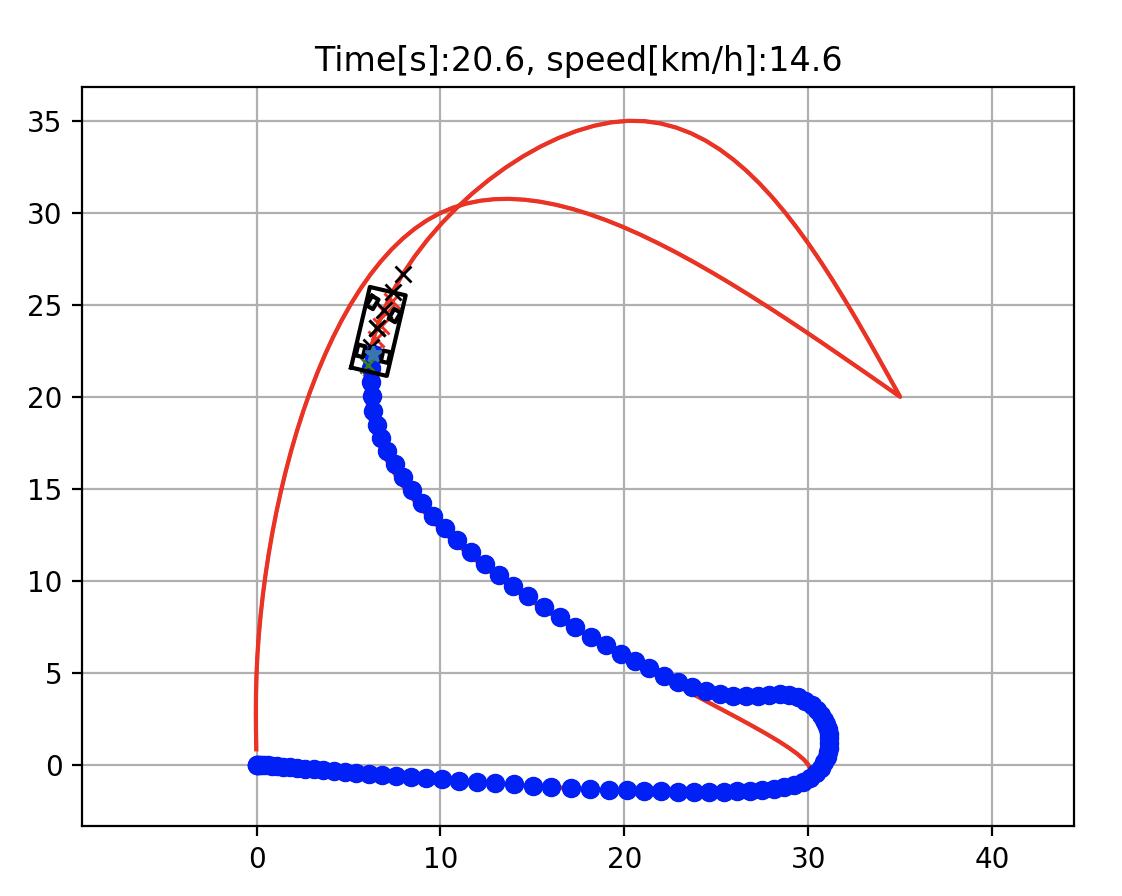
\includegraphics[width=6.2cm]{images/path_tracking2.png}}}\\
Rear wheel feedback steering control \\ and PID speed control \cite{pathtracking}& Iterative linear model predictive control
\end{tabular}
\caption{Path tracking simulation results}
\label{fig:pathplan}
\end{figure}

%------------------------------------------------------------------------- 
\section{Conclusion and future work}

In this paper, I introduced an OSS which is a Python code collection of robotics algorithms, especially for autonomous navigation. Related works of this project, some key ideas about this OSS project, and brief structure of this repository were described. 

The future works of this project is as followed: 

\begin{itemize}
 \item Technical and mathematical documentation with Jupyter notebook\cite{JupyterNotebook}.  
 \item Simple image processing samples for autonomous navigation only using OpenCV\cite{opencv}.
 \item Simple multi-robots simulations.
\end{itemize}

If readers were interested in these future projects, contributions are welcome.



%------------------------------------------------------------------------
\section{Acknowledgments}

I appreciate all contributors: Daniel Ingram\cite{auther1}, Joe Dinius\cite{auther2}, Karan Chala\cite{auther3}, Antonin RAFFIN\cite{auther4}, and Alexis Paques\cite{auther6}. This is my GitHub account\cite{auther5}

\bibliography{egbib}
\end{document}
